\section{Exact algorithms}

During the internship, we developed two exact algorithms. The first one is time efficient but has a huge memory cost, and the second one is memory efficient but is quite time consuming.

\subsection{A time efficient exact algorithm}

We first show a preliminary version of our algorithm: Algorithm \ref{algo:ckcom1} which works by doing a single pass over the $k$-cliques and by storing all $(k-1)$-cliques that are contained in a $k$-clique. It relies on the fact that the output of CPM is a partition of the $k$-cliques of the input graph such that two 
$k$-cliques are in a same partition's cluster if they share $(k-1)$-nodes: a partition's cluster is thus a connected component in the graph where nodes are $k$-cliques and two $k$-cliques are connected if they share $(k-1)$ nodes.

Thus to compute all $k$-clique communities it suffice to list all $k$-cliques while merging the communities of two $k$-cliques when they 
share a $(k-1)$-clique.

\vspace{0.3cm}

\noindent {\bf Implementation issues.} Algorithm \ref{algo:ckcom1} can be implemented efficiently by listing all $k$-cliques in the input graph using efficient algorithm such as \cite{chiba1985arboricity}; storing all $(k-1)$-cliques (contained in a $k$-clique) and using a Union-Find data structure\footnote{\url{https://en.wikipedia.org/wiki/Disjoint-set_data_structure}.}. Given a Union-Find data structure $\tt UF$ containing $n$ elements, the following two operations are allowed.
\begin{itemize}
\item ${\tt UF.Find}(a)$ returns the partition's cluster ID of element $a$ in $O(\alpha(n))$ time where $\alpha$ is the inverse Ackermann function which is essentially constant.
\item ${\tt UF.Union}(p,q)$ merges the two clusters $p$ and $q$ in $O(\alpha(n))$ time and returns the ID of the resulting cluster.
{\color{red} As $p$ and $q$ are not
elements, they are clusters IDs, so
should Union complexity be $O(1)$ ? }

\item ${\tt UF.MakeSet}(a)$ creates a new cluster and assigns $a$ to it while returning the cluster ID in constant time.
\end{itemize}
In order to have a more concise pseudocode, we also define ${\tt UF.FindOrCreate}(a)$ which returns the partition's cluster ID of element $a$ and if $a$ is not in $\tt{UF}$ it creates a new cluster and assigns $a$ to it while returning the cluster ID.

%In addition for each cluster in the partition of the $(k-1)$-cliques, we also store the set of nodes in that cluster, these overlapping clusters of nodes is the output of our algorithm.
\vspace{0.3cm}

\begin{algorithm}[!htbp]
\caption{One pass over $k$-cliques, storing $(k-1)$-cliques}
\label{algo:ckcom1}
\begin{algorithmic}[1]
  \State ${\tt UF} \leftarrow$ Union-Find datastructure 
    \For {each $k$-clique $c_k \in G$}
        \State $p \leftarrow NULL$
    	\For {each $(k-1)$-clique $c_{k-1}$ in $c_k$}
      		\State $q\leftarrow {\tt UF.FindOrCreate} (c_{k-1})$
          	\State $p \leftarrow {\tt UF.Union}(p,q) $\Comment{Returns $q$ if $p=NULL$}
      	\EndFor
    \EndFor
\end{algorithmic}
\end{algorithm}

Algorithm~\ref{algo:ckcom1} needs to store all $(k-1)$-cliques (contained in a $k$-clique) of the input graph. As the number of such $(k-1)$-cliques can be very large, this algorithm is problematic in some cases as it uses too much memory.

We next show how to avoid storing all these $(k-1)$-cliques. In particular, instead of storing the communities each $k$-clique belongs to, we store the communities each edge belongs to and we use a new datastructure that we call {\it Overlapping Union-Find} (OUF). This new datastruture builds on top of Union-Find and allows to do the same operations considering overlapping sets rather than a partition (i.e. non-overlapping sets).

We first detail how our datastructure works and then depict two pseudocodes:
\begin{itemize}
\item Algorithm \ref{algo:ckcom2} is very similar to Algorithm \ref{algo:ckcom1}, but is using an OUF instead of a UF. This 
\todo{which ? Algo1 ?}
algorithm creates a variable for each $(k-1)$-cliques found and is thus not efficient in terms of memory like Algorithm \ref{algo:ckcom2}. We show it for illustration purpose only.
\item Algorithm \ref{algo:ckcom3} is our final algorithm also using an OUF. This algorithm does not create a variable for each $(k-1)$-cliques and is much more efficient than our two first algorithms.
\end{itemize}

As we will see in Section~\ref{sec:analysis} and in Section~\ref{sec:experiments}, in addition of being orders of magnitude faster than the state-of-the-art, our final algorithm (Algorithm~\ref{algo:ckcom3}) is very efficient in terms of memory consumption. This allows our program to solve the problem for unprecedented values of $k$ and sizes of graphs using a commodity machine.

\vspace{0.3cm}

{\color{red}
OUF is a known data structure ?
If not we should explain in more details,
especially prove stuff about the complexity.
}
\noindent {\bf Overlapping Union-Find.} Given an Overlapping Union-Find data structure $\tt OUF$, we denote by $n$ the number of overlapping clusters in $\tt OUF$ and given an element 
$a$, $n_a$ denotes the number of clusters $a$ belongs to. 
The following operations are allowed.
\begin{itemize}
\item ${\tt OUF.Find}(a)$ returns the set of clusters that element $a$ belongs to in time $O(n_a\cdot\alpha(n))$;
\item $OUF.Union(p,q)$ merges the two clusters $p$ and $q$ in time $O(\alpha(n))$;
{\color{red} As $p$ and $q$ are not
elements, they are clusters IDs, so
should Union complexity be $O(1)$ ? }


\item $OUF.MakeSet()$ creates an empty cluster and returns it in time $O(1)$ and
\item $OUF.Add(a,p)$ add element $a$ to cluster $p$ (do nothing if $a$ is already in $p$) in time $O(1)$.
\end{itemize}

\todo{These operations are allowed by storing variables representing the overlapping clusters in a Union-Find datastructure and by pointing each element to the clusters that it belongs to.}

In order to have a clearer and more concise pseudocodes, we generalize the operations on sets of elements or clusters. In particular, the following operations are allowed.\\
Used in Algorithm \ref{algo:ckcom2}:
 \begin{itemize}
  \item ${\tt OUF.FindOrCreate}(A)$ returns the intersection of the sets of clusters of the elements in $A$: (i) if the intersection is a singleton, it returns a single cluster; (ii) if the intersection is empty, it creates a new cluster and add all elements in $A$ to it while returning its ID.
 \end{itemize}
Used in Algorithm \ref{algo:ckcom3}:
 \begin{itemize}
  \item ${\tt OUF.Find}(A)$ returns the intersection of the sets of clusters of the elements in $A$: (i) it returns a single cluster if the intersection is a singleton; (ii) it returns $NULL$ if the intersession is empty;
  
{  \color{red}
Hi, I propose to simplify and say just that 
it "returns the intersection of the sets of clusters of the elements in $A$." replacing lines 5-7 by only one line

        $S \leftarrow S \cup {\tt OUF.Find}(E(c_{k-1}))$
}
  \item $OUF.UnionOrCreate(P)$ merges all clusters in $P$ into a single one and returns the ID of the resulting cluster, if $P$ is empty it creates a new empty cluster and returns its ID.
  \item $OUF.Add(A,p)$ add all elements in $A$ to cluster $p$ (do nothing for an element already in $p$).
\end{itemize}

Note that following this description of operations, in line 5 of Algorithm~\ref{algo:ckcom2}, 
${\tt OUF.FindOrCreate}(E(c_{k-1}))$ always returns a single cluster and in line 5 of Algorithm~\ref{algo:ckcom2}, ${\tt OUF.Find}(E(c_{k-1}))$ always returns a single cluster or $NULL$ 
as the set of all edges belonging to a given $(k-1)$-clique can only belong to a single community.
\vspace{0.3cm}

\begin{algorithm}[!htbp]
\caption{One pass over $k$-cliques, storing edges}
\label{algo:ckcom2}
\begin{algorithmic}[1]
  \State ${\tt OUF} \leftarrow$ Overlapping Union-Find datastructure 
    \For {each $k$-clique $c_k \in G$}
        \State $q \leftarrow NULL$
    	\For {each $(k-1)$-clique $c_{k-1}$ in $c_k$}
      		\State $p \leftarrow {\tt OUF.FindOrCreate} (E(c_{k-1}))$
          	\State $q \leftarrow {\tt OUF.Union} (p,q) $ \Comment{Returns $q$ if $p=NULL$}
      	\EndFor
\EndFor
\end{algorithmic}

\end{algorithm}

\begin{algorithm}[!htbp]
\caption{One pass over $k$-cliques, storing edges}
\label{algo:ckcom3}
\begin{algorithmic}[1]
\State $OUF \leftarrow$ Overlapping Union-Find datastructure 
\For {each $k$-clique $c_k \in G$}
	\State $S\leftarrow \emptyset$
	\For {each $(k-1)$-clique $c_{k-1}$ in $c_k$}
        \State $p \leftarrow {\tt OUF.Find}(E(c_{k-1}))$%\Comment{setID containing all edges in $E$}
        \If {$p\neq NULL$}
        	\State $S \leftarrow S\cup \{p\}$
        \EndIf
    \EndFor
    \State $q\leftarrow {\tt OUF.UnionOrCreate}(S)$
	\State ${\tt OUF.Add}(E(c_k),q)$ 
\EndFor
\end{algorithmic}
\end{algorithm}


{\color{red} 
Algo 2 and 3 produce exactly the same result !
}
%Note that for $k=3$, 

\begin{figure}
    \centering
  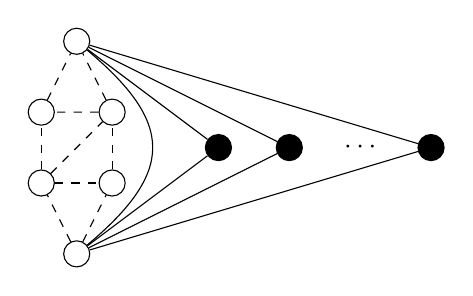
\begin{tikzpicture}[scale=0.9,rotate=90]
    \tikzstyle{w} = [circle, draw, fill=white,
    scale=1.0];
    \tikzstyle{b} = [circle, draw, fill=black,
    scale=1.0];
    \tikzstyle{gd} = [black,dashed,-];

    \node[w] (1) at (0,0){};
    \node[w] (2) at (1,0.5){};
    \node[w] (3) at (1,-0.5){};
    \node[w] (4) at (2,0.5){};
    \node[w] (5) at (2,-0.5){};
    \node[w] (6) at (3,0){};

    \node[b] (7) at (1.5,-2){};
    \node[b] (8) at (1.5,-3){};
    \node[] (9) at (1.5,-4){$\cdots$};
    \node[b] (9) at (1.5,-5){};

    \path[gd] (1) edge (2)
                  edge (3)
              (2) edge (3)
                  edge (4)
                  edge (5)
              (3) edge (5)
              (4) edge (6)
              (5) edge (6)
                  edge (4);
                  
    \path[-]  (1) edge [bend right=50,
                        looseness = 1.5] (6);
    \path[-]  (7) edge (1)
                  edge (6)
              (8) edge (1)
                  edge (6)
              (9) edge (1)
                  edge (6);
                  


  \end{tikzpicture}
    \caption{A problematic graph for algorithm 
    that stores only nodes CPM0.
    It merges dashed and black triangle 
    communities if any 
    black clique is considered after 
    all cliques of the dashed community.
    The number of black cliques
    can be arbitrary large, 
    implying that CPM0 with 
    a random order of clique 
    processing will almost surely merge two 
    communities when the number of black cliques
    tends to infinity.
    Our approximate
    Algorithms~\ref{algo:ckcom2}
    and~\ref{algo:ckcom3} 
    stores links not just nodes. 
    They are immune to this problematic case.
    }
    \label{gr0}
\end{figure}

\begin{figure}
    \centering
  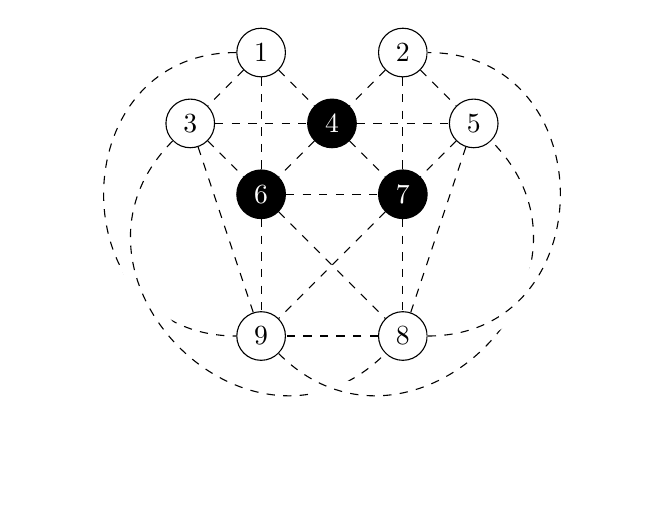
\begin{tikzpicture}[scale=0.9, rotate=0]
   \tikzstyle{nod1} = [circle, draw, fill=black, scale=1.0,
                       text = white];
   \tikzstyle{nod2} = [circle, draw, fill=white, scale=1.0];
   \tikzstyle{gd} = [black,dashed,-];

    \node[nod2] (1) at  (0,0){1};
    \node[nod2] (2) at  (2,0){2};
    
    \node[nod2] (3) at  (-1,-1){3};
    \node[nod1] (4) at  (1,-1){4};
    \node[nod2] (a5) at  (3,-1){5};
    \node[nod1] (a6) at  (0,-2){6};
    \node[nod1] (a7) at  (2,-2){7};
    \node[nod2] (a8) at (2,-4){8};
    \node[nod2] (a9) at (0,-4){9};
    
    \path[gd] (1) edge  (3);
    \path[gd] (1) edge  (4);
    \path[gd] (1) edge  (a6);
    
    \path[gd] (2) edge  (a5);
    \path[gd] (2) edge  (4);
    \path[gd] (2) edge  (a7);
    \path[gd] (3) edge  (4);
    \path[gd] (3) edge  (a6);

    \path[gd] (4) edge  (a6);
    \path[gd] (4) edge  (a7);
    \path[gd] (4) edge  (a5);
    
    \path[gd] (a5) edge  (a7);

    \path[gd] (a6) edge  (a7);
    \path[gd] (a6) edge  (a9);
    \path[gd] (a6) edge  (a8);
    
    \path[gd] (a7) edge  (a9);
    \path[gd] (a7) edge  (a8);


    %% links of a clique from another community
    % \path[thick] (4) edge  (5);
    % \path[thick] (a7) edge  (5);
    % \path[thick] (a6) edge  (5);

    \path[gd] (3) edge (a9);
    \path[gd] (a5) edge (a8);
    
    \path[gd] (1) edge 
    [bend right=90, looseness=1.6] (a9);
    
    \path[gd] (a9) edge 
    [bend right=90, looseness=1.6] (a5);

    \path[white,-] (3) edge 
    [bend right=90, looseness=1.6, line width=3mm
    ] (a8);
    \path[gd] (3) edge 
    [bend right=90, looseness=1.6] (a8);

    \path[white,-] (a9) edge 
    [bend right=90, looseness=1.6, line width=3mm
    ] (a5);
    \path[gd] (a9) edge 
    [bend right=90, looseness=1.6] (a5);

    \path[white,-] (a8) edge
    [bend right=90, looseness=1.6, line width=3mm
    ] (2);
    \path[gd] (a8) edge 
    [bend right=90, looseness=1.6] (2);

    
    \path[gd] (a8) edge  (a9);
    
  \end{tikzpicture}
    \caption{
    A $(k-1)$-clique $F$ is called {\em phantom}
    if it is contained in a (sub)graph covered by a 
    $k$-clique percolation denoted by $P$ but 
    there is no $k$-clique in $P$ that contains $F$.
    %    Alexis Baudin's definition 
    % Etant donné une percolation de 
    % k-cliques sur un graphe, une 
    % communauté est un ensemble de 
    % k-cliques.     Une **(k-1)-clique 
    % parasite** de cette communauté est une
    % (k-1)-clique qui apparait dans le 
    % graphe de la communauté mais qui 
    % n'appartient à aucune clique de la 
    % communauté.
    This figure represents a minimal example
    of a graph covered by a $k$-clique percolation
    and containing a phantom $(k-1)$-clique,
    for $k = 4$. Duplicating a node from the clique
    one can easily generate an additional
    phantom clique.
    }
    \label{gr0}
 \end{figure}



We now proceed to the theoretical analysis of our algorithms.



\subsection{A memory efficient exact algorithm}

A community is a set of $k$-cliques. Keeping in memory all its $k$-cliques, or all its $(k-1)$-cliques, is not scaling well for huge graphs. A way of tackling this issue is to find a way to compress the data. In this section, the main idea is to store a community as a graph, storing only the nodes and the edges of the $k$-cliques added. So, we say that a $k$-clique is in the community if all its nodes and edges are in the community. Consequently, it can happen that a $k$-clique is tested beeing in the community whereas it has not be added to it. So, the community appears to have more $k$-clique that should be. The main issue is that if a $k$-clique appears to be in a community, and is also in another one, the two communities are merged, whereas it should not.

Therefore, whereas keeping the community as a list of edges allows to store communities with few memory, it creates parasites cliques that we need to compute and to store. A $k$-clique is added to the community if it shares a $(k-1)$-clique with it. A $(-1)$-clique parasite of a community is a $(k-1)$-clique that is tested to be in the community but which is not part of any $k$-clique added to the community. In consequence, if the $(k-1)$-clique common to a $k$-clique and a community is a parasite, we need to know it not to add the $k$-clique to the community.

In consequence, we choose to use a procedure to list all the $(k-1)$-cliques parasites of a community. Every time an edge  is added to the community, we list all the $(k-1)$-cliques of the community containing this edge. Each one which is not a sub-clique of the $k$-clique added is then a parasite $(k-1)$-clique (RESULTAT A METTRE EN VALEUR ? + PREUVE ?). Then, we remove all the $(k-1)$-subliques of the $k$-clique added, so the list of $(k-1)$-cliques parasites is always up-to-date.

\begin{algorithm}
  \caption{CPM 3 condensé}
  \begin{algorithmic}[1]
    \State GraphCommus $\gets dict()$ % \Comment{Graphs of communities}
    \State GhostCliques $\gets dict()$ % \Comment{Ghost cliques of communities}
    \State Fusions $\gets []$ % \Comment{Fusions to perform at the end of the algorithm}
    \For{each $k$-clique $c_k \in G$}
    \State commus\_ck $\gets$ \Call{CommusNeighboursOf}{$c_k$, GraphCommus, GhostCliques}
    %\State
    \If{commus\_ck == $\emptyset$} %\Comment{No current community is a neighbour of $c_k$}
    \State \Call{CreateCommu}{$c_k$, GraphCommus, GhostCliques} \Comment{$c_k$ : new community}
    %\State
    \Else \Comment{Pick one neighbour community and add $c_k$ to it, computing new ghost cliques for each new edge}
    \State $commu$ $\gets$ ONE community from commus\_ck
    \State \Call{AddToCommuGraph}{$c_k$, GraphCommus, GhostCliques}
    \If{|commus\_ck| > 1} \Comment{Record the other communities to merge them at the end}
    \State Fusions.push(commus\_ck) 
    \EndIf
    \EndIf
    \EndFor
    %\State 
    \State \Call{ApplyFusions}{Fusions, GraphCommus}
  \end{algorithmic}
\end{algorithm}